\begin{itemize}
 \item \textbf{Input:} $n$ activities $a_1, \cdots, a_n$, where $a_i$ starts at 
time $x_i$ and ends at time $y_i$.
\item \textbf{Feasible Solution:} Any subset of these activities such that no 
two activities in the subset overlap. 
\item \textbf{Objective Function:} Maximize the number of activities we 
schedule.
\end{itemize}

\subsection{Some Attempts}
Criterions to be greedy on:
\begin{itemize}
	\item Pick the activities with shortest duration. 
	
	It dose not work. The counter example is as follows:
    \begin{figure}[H]
    \centering
    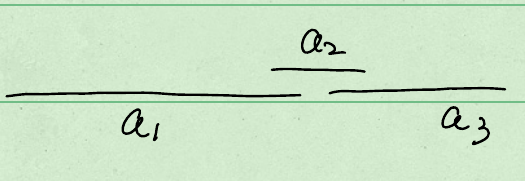
\includegraphics[width=0.3\textwidth]{1st-attempt.png}
    \end{figure}
	\item Pick the activities what finish first.\\
        Sort the activities by finish time and then renumber them so that $f_1 
\le f_2 \cdots \le f_n$
\end{itemize}
\subsection{Proposed Greedy Algorithm}
Given a set of activities, 
\begin{itemize}
	\item Pick the earliest finishing activities that remain.
	\item Remove all activities that conflict with the chosen activity.
	\item Repeat.
\end{itemize}

To prove the correctness, we start by arguing that the algorithm 
is not wrong on its first choice.

\begin{claim}
	\textbf{Greedy Choice Property:} First choice made by greedy algorithm is 
not wrong.
\end{claim}
To be more specific, in activities selection problem, if greedy algorithm 
choose an activity at first, then there is an optimal feasible solution that 
contain $a_1$.

\begin{claimproof}
	Suppose for contradiction that no optimal feasible solution uses $a_1$. 
Let $O$ be the subset of activities in some optimal solution. We can order the 
activities in $O$ by finish time.

    Let $a_{i1}, a_{i2}, \cdots, a_{ik}$ be the activities in $O$ so ordered. 
We can make an \textbf{exchange argument} as the following plot. Throw out 
$a_i$ from $O$ and include $a_1$ in instead to get a new set of activities 
$O'$. 

    There are some properties about $O'$.
    \begin{itemize}
        \item $|O'| = |O|$
        \item $O'$ is feasible.
        \item $O'$ is also optimal and contains $a_1$. 
$\Rightarrow\mskip-\thinmuskip\Leftarrow$
    \end{itemize}

    \begin{figure}[H]
    \centering
    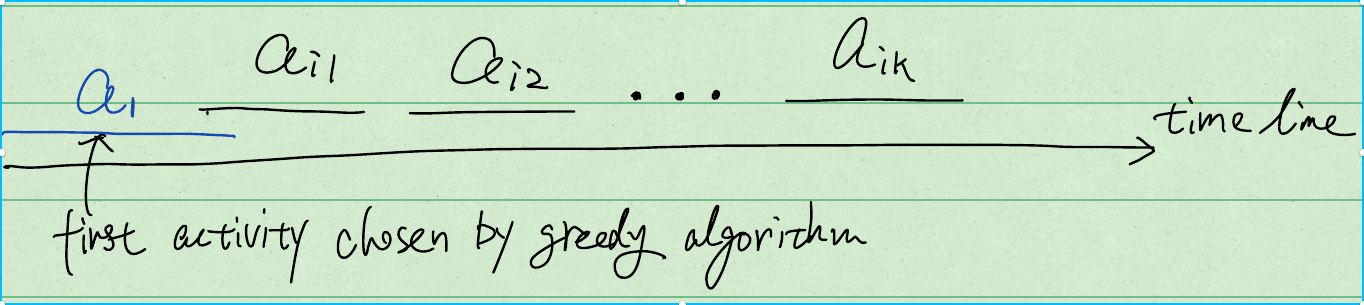
\includegraphics[width=0.5\textwidth]{exchange-selection-1.png}
    \end{figure}
\end{claimproof}

There is a way to construct an optimal solution starting with $a_1$. This 
optimal solution should certainly exclude activities that conflict with $a_1$. 
Recursively need to solve a smaller problem consisting of activities that do 
not conflict with $a_1$. In particular, the smaller problem is finding the 
optimal subset of activities out of the remaining activities.

\begin{claim}
    \textbf{Optimal Substructure Property}
	In the set of activities, we need to pick an optimal feasible 
subset activities.
\end{claim}
\begin{claimproof}{}
\begin{itemize}
	\item $A$: Original set of activities
	\item $A'$: Set of activities that remain after throwing out $a_1$ and 
its conflicting activities.
\end{itemize}
    Any solution to $A'$ that gives value $k$ can be extended to a solution to 
$A$ of value $(k+1)$ by adding $a_1$. So need optimal solution to $A'$
\end{claimproof}

In general. Optimal Substructure Property inductively assumes that greedy 
solves problem with fewer than $n$ activities optimally.

Greedy Choice Property and Optimal Substructure Property imply that greedy 
solve $n$-activity problem optimally.

\subsubsection{Time}
We sort the activities by finish time take $O(n\log n)$. Then the rest of steps 
can be done in linear or constant time.
